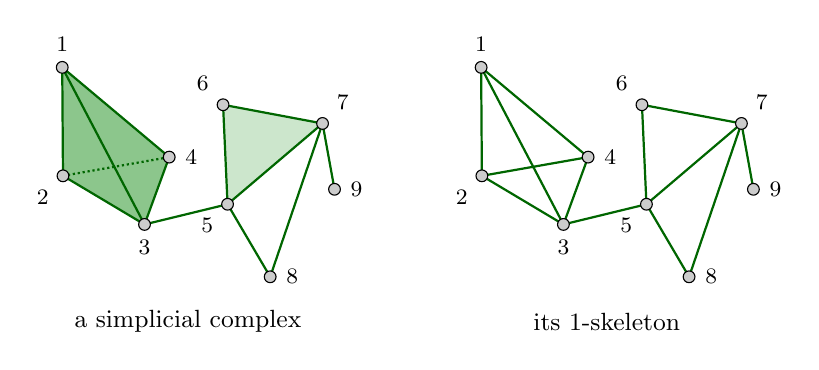
\begin{tikzpicture}[scale=0.95, font=\small,
  vtx/.style={circle, draw=black, fill=gray!40, inner sep=1.5pt}]
\foreach \dx/\title/\full in {0/{a simplicial complex}/1, 5.6/{its 1-skeleton}/0} {
\begin{scope}[xshift=\dx cm]
  \coordinate (v1) at (0.72,2.80);
  \coordinate (v2) at (0.73,1.35);
  \coordinate (v3) at (1.82,0.70);
  \coordinate (v4) at (2.15,1.60);
  \coordinate (v5) at (2.93,0.97);
  \coordinate (v6) at (2.87,2.30);
  \coordinate (v7) at (4.20,2.05);
  \coordinate (v8) at (3.50,0.00);
  \coordinate (v9) at (4.36,1.17);
  \ifnum\full=1
    % solid tetrahedron {1,2,3,4} and filled triangle {5,6,7}
    \fill[green!50!black, opacity=0.45] (v1) -- (v2) -- (v3) -- (v4) -- cycle;
    \fill[green!50!black, opacity=0.2] (v5) -- (v6) -- (v7) -- cycle;
    \draw[thick, green!40!black] (v1) -- (v2) -- (v3) -- (v4) -- cycle (v1) -- (v3);
    \draw[thick, green!40!black, densely dotted] (v2) -- (v4);
  \else
    \draw[thick, green!40!black] (v1) -- (v2) -- (v3) -- (v4) -- cycle (v1) -- (v3) (v2) -- (v4);
  \fi
  \draw[thick, green!40!black] (v3) -- (v5) (v5) -- (v6) -- (v7) -- cycle
    (v5) -- (v8) -- (v7) (v7) -- (v9);
  \foreach \i/\pos in {1/above, 2/below left, 3/below, 4/right, 5/below left, 6/above left, 7/above right, 8/right, 9/right}
    \node[vtx, label={[font=\footnotesize]\pos:\i}] at (v\i) {};
  \node at (2.4,-0.6) {\title};
\end{scope}
}
\end{tikzpicture}
